\ifgerman{\chapter{Evaluierung}}{\chapter{Evaluation}}
\label{ch:evaluation}

Evaluating a classification algorithm also known as classification model is necessary to find how competent the algorithm is on data it has never seen. The classification model generates probabilities when given the of predicting on unobserved data. 

\section{Experimental Setup}
Most of the experiments were carried out on \textit{Google Colab} is a free Google service that provides Jupyter notebooks with Python environment that stores the notebooks on Google Drive. It provides a GPU (Graphics Processing Unit) or TPU (Tensor Processing Unit) and has pre-installed various popular machine learning and deep learning framework. The exact detail of the system is listed in the \ref{table:HWsetup}

\begin{table}[!ht]
\centering
\begin{tabular}{cc}
\hline
\textbf{Hardware} & \textbf{Specifications} \\ \hline
CPU & 2vCPU Intel(R) Xeon(R) Processors @2.20Ghz \\
GPU & 1xTesla K80 12GB(11.439GB Usable) GDDR5  VideoRAM \\
TPU & \multicolumn{1}{l}{Google's custom developed application-specific integrated circuits} \\
RAM & 12GB \\
DISK & 358.27 GB \\ \hline
\end{tabular}
\captionsetup{justification=justified,margin=1cm}
\caption{Hardware specification for the experimental setup}
\label{table:HWsetup}
\end{table}

All the experiments were performed using \textit{Python 3} environment. \textit{scikit-learn}, an open source machine learning library in Python is used here for data processing and training the SVM. For \glspl{BiLSTM}, \textit{Keras} an open source neural network library written in Python is used with \textit{Tensorflow} backend.  

The packages, their version numbers and the description of the packages are listed below in \ref{tabel:packageList}
\clearpage
\begin{table}[!ht]
\centering
\begin{tabular}{>{\centering\arraybackslash}m{3.4cm}>{\centering\arraybackslash}m{3.4cm}>{\centering\arraybackslash}m{6cm}}
\hline
\textbf{Package Name} & \textbf{Version Number} & \textbf{Description} \\ \hline
scikit-learn & 0.20.3 & An open source machine learning library for data mining and data analysis. \\[0.2cm]
keras & 2.2.4 & An open source neural network library for fast prototyping, uses likes of Tensorflow or Theano. \\[0.2cm]
tensorflow & 1.13.1 & An open source software library for numerical computation using data flow graphs. \\[0.2cm]
beautifulsoup4 & 4.6.3 & A python library for parsing HTML and XML documents. \\[0.2cm]
matplotlib & 3.0.3 & A python library for plotting and visualization. \\[0.2cm]
nltk & 3.2.5 & A python library for statistical Natural Language Processing. \\[0.2cm]
seaborn & 0.7.1 & A python library for statistical data visualization. \\[0.2cm]
spacy & 2.0.18 & An open-source software library for advanced Natural Language Processing. \\[0.2cm]
numpy & 1.14.6 & An python library for creating and manipulating, large and multiple dimensional arrays. \\[0.2cm]
scipy & 1.1.0 & An python library for scientific and technical computing. \\ [0.2cm] 
Fasttext & 0.2.0 & An python library for training word vectors. \\ [0.2cm]
MUSE & NA & A library for aligning word vectors into a single vector space. \\ [0.2cm]
XlingualEmb & NA & A library for learning bilingual word vectors.  \\  \hline
\end{tabular}
\captionsetup{justification=justified,margin=1cm}
\caption{List of packages used}
\label{tabel:packageList}
\end{table}


\section{Evaluation Approach}
For evaluation, initially 70\% of data is used for training the classification models, and then 30\% of the data is used for evaluating it. The evaluation is done on sentence level and on document level \ref{evaluationQuestionOne} using performance evaluation matrices described in \ref{backgroundEvaluationMatrices}. The evaluation of each question will go in detail about the performance of each classification model. Beside the described performance evaluation matrices, as the dataset used for training is an imbalanced one, the evaluation will also go into the details about the performance of the classifiers on each class in order to get better insights of how well it is performing for the underrepresented classes (the minority classes).


\subsection{Evaluation for the first research question} \label{EvalQ1}

The first research question compares the performance of \gls{SVM} and \gls{BiLSTM} trained on English corpus. It also evaluates the classification performance of \gls{BiLSTM} trained on unclustered bilingual corpora compared with the one trained on clustered bilingual corpora.  

Before training the \gls{SVM}, we had to find the value of $C$, which we found to be 1 among all other values.

The \ref{fig:question1EvalMicro} shows the Micro-average and \ref{fig:question1EvalMacro} shows the Macro-average performance of different classifiers evaluated on sentence and document level. The results of the algorithm trained on clustered data are averaged together as mention in \ref{evaluationQuestionOne}

%%%%%%%%%%%%%%%%%%%%%%%%%%%%%  MACRO AVERAGE BAR CHART %%%%%%%%%%%%%%%%%%%%%%%%%%%%%%%%%%%%%%%%%%%%%%%%%%%%%%%%%%%%%%%%
\begin{figure}[!ht]
    \centering
    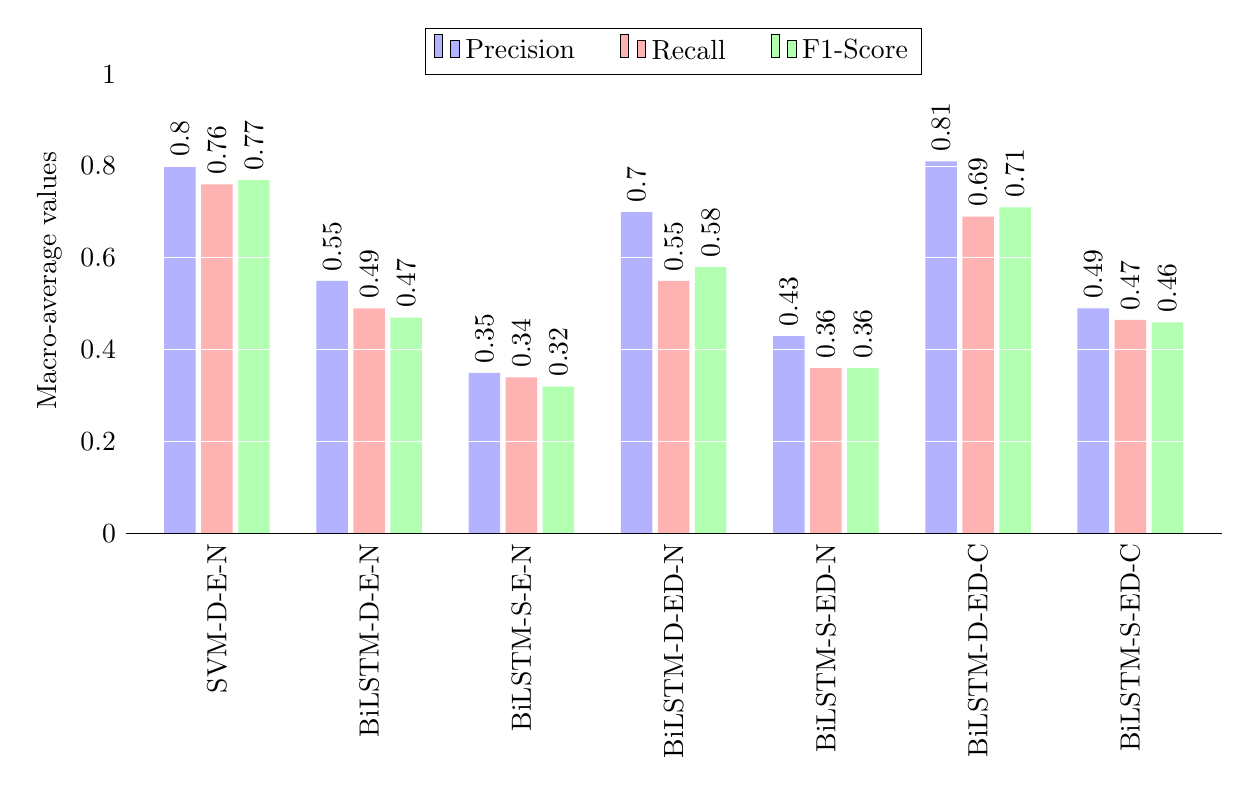
\begin{tikzpicture}
          \begin{axis}[
              ybar, axis on top,
              height=8cm, width=15.5cm,
              bar width=0.4cm,
              ymajorgrids, tick align=inside,
              major grid style={draw=white},
              enlarge y limits={value=.1,upper},
              ymin=0, ymax=1,
              axis x line*=bottom,
              axis y line*=left,
              x tick label style={rotate=90,anchor=east},
              y axis line style={opacity=0},
              tickwidth=0pt,
              enlarge x limits=true,
              legend style={
                  at={(0.5, 1)},
                  anchor=north,
                  legend columns=-1,
                  /tikz/every even column/.append style={column sep=0.5cm}
              },
              ylabel={Macro-average values},
              symbolic x coords=
              {
              SVM-D-E-N,
              BiLSTM-D-E-N,
              BiLSTM-S-E-N,
              BiLSTM-D-ED-N,
              BiLSTM-S-ED-N,
              BiLSTM-D-ED-C,
              BiLSTM-S-ED-C
              },
             xtick=data,
             nodes near coords,        
             every node near coord/.append style={color=black,rotate=90, anchor=west }
             %nodes near coords={
             %\pgfmathprintnumber[precision=1]{\pgfplotspointmeta}
             %}
          ]
          \addplot [draw=none, fill=blue!30] coordinates   % Precision Values for all the models
          {
              (SVM-D-E-N,0.8)
              (BiLSTM-D-E-N,0.55)
              (BiLSTM-S-E-N,0.35)
              (BiLSTM-D-ED-N,0.7)
              (BiLSTM-S-ED-N,0.43)
              (BiLSTM-D-ED-C,0.81)
              (BiLSTM-S-ED-C,0.49)
            
          };
         \addplot [draw=none,fill=red!30] coordinates  % Recall Values for all the models
          {
              (SVM-D-E-N,0.76)
              (BiLSTM-D-E-N,0.49)
              (BiLSTM-S-E-N,0.34)
              (BiLSTM-D-ED-N,0.55)
              (BiLSTM-S-ED-N,0.36)
              (BiLSTM-D-ED-C,0.69)
              (BiLSTM-S-ED-C,0.465)    
          };
         \addplot [draw=none, fill=green!30] coordinates % F1-Score Values for all the models
          {
              (SVM-D-E-N,0.77)  
              (BiLSTM-D-E-N,0.47)
              (BiLSTM-S-E-N,0.32)
              (BiLSTM-D-ED-N,0.58)
              (BiLSTM-S-ED-N,0.36)
              (BiLSTM-D-ED-C,0.71)
              (BiLSTM-S-ED-C,0.46)
            
          };
        
          \legend{Precision, Recall, F1-Score}
        \end{axis}
        \end{tikzpicture}
        \captionsetup{justification=justified,margin=1cm}
    \caption{Macro-averaged \textit{Precision}, \textit{Recall} and \textit{F1-Score} of \gls{SVM} and \gls{BiLSTM} in different configurations. The first suffix D or S indicates evaluation on document or sentence level respectively, the second suffix E or D represents the language of the corpus used respectively. The third suffix N or C indicates non clustered and clustered respectively.}
    \label{fig:question1EvalMacro}
\end{figure}
%%%%%%%%%%%%%%%%%%%%%%%%%%%%%%%%%%%%%%%%%%%%%%%%%%%%%%%%%%%%%%%%%%%%%%%%%%%%%%%%%%%%%%%%%%%%%%%%%%%%%%%%%%%%%%%%%%%%%%%

%%%%%%%%%%%%%%%%%%%%%%%%%%%%%%%%%%%%%%%%%% MICRO-AVERAGE BAR CHART %%%%%%%%%%%%%%%%%%%%%%%%%%%%%%%%%%%%%%%%%%%%%%%%%%%%

\begin{figure}[!ht]
    \centering
     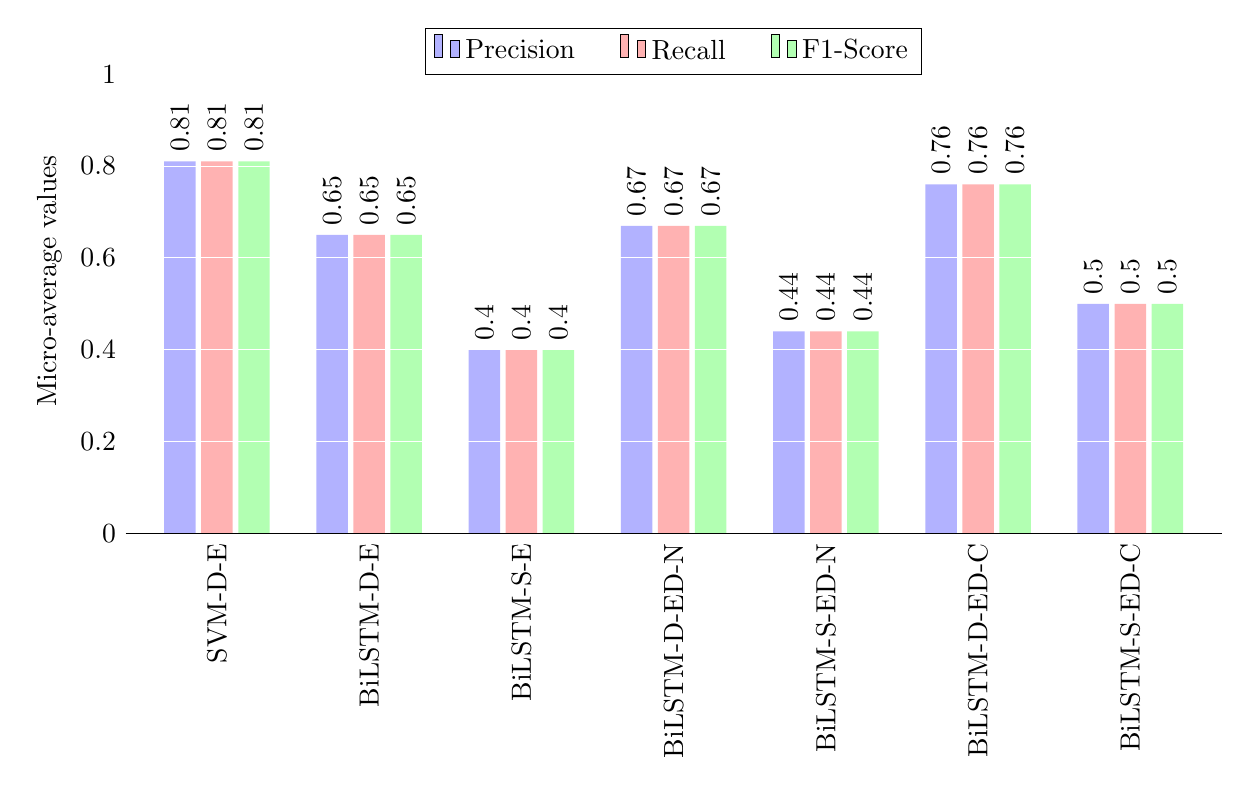
\begin{tikzpicture}
  \centering
  \begin{axis}[
        ybar, axis on top,
        height=8cm, width=15.5cm,
        bar width=0.4cm,
        ymajorgrids, tick align=inside,
        major grid style={draw=white},
        enlarge y limits={value=.1,upper},
        ymin=0, ymax=1,
        axis x line*=bottom,
        axis y line*=left,
        x tick label style={rotate=90,anchor=east},
        y axis line style={opacity=0},
        tickwidth=0pt,
        enlarge x limits=true,
        legend style={
            at={(0.5, 1)},
            anchor=north,
            legend columns=-1,
            /tikz/every even column/.append style={column sep=0.5cm}
        },
        ylabel={Micro-average values},
        symbolic x coords=
        {
        SVM-D-E,
        BiLSTM-D-E,
        BiLSTM-S-E,
        BiLSTM-D-ED-N,
        BiLSTM-S-ED-N,
        BiLSTM-D-ED-C,
        BiLSTM-S-ED-C
        },
       xtick=data,
       nodes near coords,        
       every node near coord/.append style={color=black,rotate=90, anchor=west }
       %nodes near coords={
       %\pgfmathprintnumber[precision=1]{\pgfplotspointmeta}
       %}
    ]
   \addplot [draw=none, fill=blue!30] coordinates   % Precision Values for all the models
    {
        (SVM-D-E,       0.81)
        (BiLSTM-D-E,    0.65)
        (BiLSTM-S-E,    0.4)
        (BiLSTM-D-ED-N, 0.67)
        (BiLSTM-S-ED-N, 0.44)
        (BiLSTM-D-ED-C, 0.76)
        (BiLSTM-S-ED-C, 0.5)
      
    };
   \addplot [draw=none,fill=red!30] coordinates  % Recall Values for all the models
    {
        (SVM-D-E,       0.81)
        (BiLSTM-D-E,    0.65)
        (BiLSTM-S-E,    0.4)
        (BiLSTM-D-ED-N, 0.67)
        (BiLSTM-S-ED-N, 0.44)
        (BiLSTM-D-ED-C, 0.76)
        (BiLSTM-S-ED-C, 0.5)    
    };
   \addplot [draw=none, fill=green!30] coordinates % F1-Score Values for all the models
    {
        (SVM-D-E,       0.81)
        (BiLSTM-D-E,    0.65)
        (BiLSTM-S-E,    0.4)
        (BiLSTM-D-ED-N, 0.67)
        (BiLSTM-S-ED-N, 0.44)
        (BiLSTM-D-ED-C, 0.76)
        (BiLSTM-S-ED-C, 0.5)    
      
    };

    \legend{Precision, Recall, F1-Score}
  \end{axis}
  \end{tikzpicture}
  \captionsetup{justification=justified,margin=1cm}
    \caption{Micro-averaged \textit{Precision}, \textit{Recall} and \textit{F1-Score} of \gls{SVM} and \gls{BiLSTM} in different configurations. The first suffix D or S indicates evaluation on document or sentence level respectively, the second suffix E or D represents the language of the corpus used respectively. The third suffix N or C indicates non clustered and clustered respectively. }
    \label{fig:question1EvalMicro}
\end{figure}

%%%%%%%%%%%%%%%%%%%%%%%%%%%%%%%%%%%%%%%%%%%%%%%%%%%%%%%%%%%%%%%%%%%%%%%%%%%%%%%%%%%%%%%%%%%%%%%%%%%%%%%%%%%%%%%%%%%%%%%%%%%%%%%%%%%%%%%%%%%%%%%



\ref{fig:question1EvalMicro} shows that the performance of the SVM is far more superior then \gls{BiLSTM} when trained only on English corpus on document level. The result of the same \gls{BiLSTM} when evaluated on a sentence level is less compared to when evaluated on document level. The results on the sentence level are significantly lower compared to the results on the document level. This behavior can be further explained by considering an example document which is categorized in class $A$ and contains three sentences. As described in the \ref{backgroundSlidingWindow} all the three sentences of this document will have the same class as the document.

\begin{table}[!ht]
\centering
\begin{tabular}{>{\centering\arraybackslash}m{3cm}>{\centering\arraybackslash}m{3cm}>{\centering\arraybackslash}m{3cm}>{\centering\arraybackslash}m{3cm}}
\hline
\textbf{Sentence Identifier} & \textbf{Prediction Score of each class, [Class A, Class B]} & \textbf{True class} & \textbf{Predicted class} \\ \hline
Sentence I & {[}0.9, 0.1 {]} & A & A \\[0.2cm]
Sentence II & {[}0.49, 0.51{]} & A & B \\[0.2cm]
Sentence III & {[}0.45, 0.55{]} & A & B \\ [0.2cm]\hline
Summation of prediction score for the whole document (normalized) & {[}0.62 , 0.38{]} & A & A
\end{tabular}
\captionsetup{justification=justified,margin=1cm}
\caption{Document with three sentences, prediction score for each class, true class and predicted class}
\label{table:SentVsDoc}
\end{table}

From the \ref{table:SentVsDoc}, we can see that the predicted score of \textit{Sentence I} for class $A$ is 0.9 and for class $B$ is 0.1, hence it is predicted in class A  but for \textit{Sentence B} and \textit{sentence C} although they belong to class $A$ they are predicted in class $B$ since the classifier was uncertain about the decision. However, when we combine the predicted score for all the classes from all the sentences and normalize them, the overall score for the document is higher for class $A$, so the precision of the above classifier on sentence level will be $\frac{1}{3} = 0.33$ and on document level the precision is $\frac{1}{1} = 1$ and therefore when evaluating on document level, the performance matrices will be better. 
\todo{Advantages of confidence values instead of heuristically assigning class label on the bases of majority vote.}

The \ref{tabel:LSTMCluster&NonClustered} shows the class-wise \textit{precision, recall} and \textit{F1-Score} values for \gls{BiLSTM} trained on English and German corpus with clustering and without clustering.


The effect of clustering is also evident from \ref{fig:question1EvalMicro} and \ref{fig:question1EvalMacro}. The specialization advantage of clustering improves the classification performance on the document level as well as on the sentence level. Also, we can see that micro-average f1-score for non clustered data in \gls{BiLSTM} on bilingual corpus is higher than macro-average values, this indicates that the performance of the classifier on minority classes on clustered data is better than non clustered data. This can be confirmed by looking at the class-wise precision, recall and f1-score values in the \ref{tabel:LSTMCluster&NonClustered} for class \textit{Audiovisual and Media} and \textit{Culture} which has 18 and 21 instances respectively (see \ref{table:befforeAfterResampling})   

The micro-average values in \ref{fig:question1EvalMicro} are same for a classifier. Hence, the calculation of the micro-average precision, recall and f1-score for BiLSTM-D-ED-C cluster 1 is done in \ref{MicroMacroCalculation} to confirm that it is indeed the same. 

\clearpage
\begin{table}[!ht]
\centering
\begin{tabular}{>{\raggedright\arraybackslash}m{5.8cm}>{\centering\arraybackslash}m{1cm}>{\centering\arraybackslash}m{1cm}>{\centering\arraybackslash}m{1cm}>{\centering\arraybackslash}m{1.1cm}>{\centering\arraybackslash}m{1.1cm}>{\centering\arraybackslash}m{1.1cm}}
\hline
Category & P$_\text{LSTM}$ &  R$_\text{LSTM}$ & F$_\text{LSTM}$ & P$_\text{LSTM-C}$ & R$_\text{LSTM-C}$ & F$_\text{LSTM-C}$ \\ \hline
Agriculture & 0.74 & 0.78 & 0.76 & \hlc[precision]{ 0.90} & \hlc[recall]{0.86} & \hlc[fscore]{0.88} \\
Audiovisual and Media & 0.00 & 0.00 & 0.00 & \hlc[precision]{ 1.00} & \hlc[recall]{0.10} & \hlc[fscore]{0.18} \\
Budget & \hlc[precision]{ 0.90} & 0.45 & 0.60 & 0.78 & \hlc[recall]{0.70} & \hlc[fscore]{0.74} \\
Competition & 0.90 & 0.63 & 0.75 & \hlc[precision]{ 0.96} & \hlc[recall]{0.83} & \hlc[fscore]{0.89} \\
Consumers & 0.54 & 0.54 & 0.54 & \hlc[precision]{ 0.59} & \hlc[recall]{0.65} & \hlc[fscore]{0.62} \\
Culture & 0.00 & 0.00 & 0.00 & \hlc[precision]{ 0.93} & \hlc[recall]{1.00} & \hlc[fscore]{0.97} \\
Customs & 0.78 & 0.47 & 0.58 & \hlc[precision]{ 0.64} & \hlc[recall]{0.70} & \hlc[fscore]{0.67} \\
Development & 0.45 & 0.81 & 0.57 & \hlc[precision]{ 0.64} & \hlc[recall]{0.83} & \hlc[fscore]{0.72} \\
Economic and Monetary Affairs & 0.85 & \hlc[recall]{0.93} & 0.89 & \hlc[precision]{ 0.95} & 0.87 & \hlc[fscore]{0.91} \\
Education Training Youth & 0.64 & 0.94 & 0.77 & \hlc[precision]{ 0.86} & 0.94 & \hlc[fscore]{0.90} \\
Employment and Social Policy & 0.68 & 0.83 & 0.75 & \hlc[precision]{ 0.71} & \hlc[recall]{0.88} & \hlc[fscore]{0.79} \\
Energy & 0.71 & \hlc[recall]{0.71} & 0.71 & \hlc[precision]{ 0.97} & 0.64 & \hlc[fscore]{0.77} \\
Enlargement & 0.70 & 0.44 & 0.54 & \hlc[precision]{ 0.76} & \hlc[recall]{0.59} & \hlc[fscore]{0.67} \\
Enterprise & 0.44 & 0.15 & 0.23 & \hlc[precision]{ 0.65} & \hlc[recall]{0.42} & \hlc[fscore]{0.51} \\
Environment & 0.69 & 0.82 & 0.75 & \hlc[precision]{ 0.70} & \hlc[recall]{0.84} & \hlc[fscore]{0.76} \\
External Relations & \hlc[precision]{ 1.00} & 0.23 & 0.37 & 0.92 & \hlc[recall]{0.55} & \hlc[fscore]{0.69} \\
External Trade & 0.53 & 0.61 & 0.57 & \hlc[precision]{ 0.61} & \hlc[recall]{0.71} & \hlc[fscore]{0.66} \\
Fight Against Fraud & \hlc[precision]{ 1.00} & 0.25 & 0.40 & 0.53 & \hlc[recall]{0.50} & \hlc[fscore]{0.52} \\
Food Safety & 0.90 & 0.82 & 0.86 & \hlc[precision]{ 0.93} & 0.82 & \hlc[fscore]{0.87} \\
Foreign and Security Policy & 0.65 & 0.54 & 0.59 & \hlc[precision]{ 0.62} & \hlc[recall]{0.83} & \hlc[fscore]{0.71} \\
Human Rights & 1.00 & 0.12 & 0.22 & \hlc[precision]{ 0.59} & \hlc[recall]{0.71} & \hlc[fscore]{0.64} \\
Humanitarian Aid & 1.00 & 0.29 & 0.44 & \hlc[precision]{ 0.67} & \hlc[recall]{0.57} & \hlc[fscore]{0.62} \\
Information Society & 0.54 & 0.72 & 0.62 & \hlc[precision]{ 0.71} & \hlc[recall]{0.84} & \hlc[fscore]{0.77} \\
Institutional Affairs & 0.62 & 0.60 & 0.61 & \hlc[precision]{ 0.67} & \hlc[recall]{0.65} & \hlc[fscore]{0.66} \\
Internal Market & 0.62 & 0.70 & 0.66 & \hlc[precision]{ 0.72} & \hlc[recall]{0.75} & \hlc[fscore]{0.74} \\
Justice Freedom Security & 0.53 & \hlc[recall]{0.86} & 0.66 & \hlc[precision]{ 0.81} & 0.67 & \hlc[fscore]{0.74} \\
Maritime Affairs and Fisheries & 0.91 & 0.80 & 0.85 & \hlc[precision]{ 0.94} & \hlc[recall]{0.91} & \hlc[fscore]{0.92} \\
Public Health & 1.00 & 0.39 & 0.56 & \hlc[precision]{ 0.86} & \hlc[recall]{0.43} & \hlc[fscore]{0.58} \\
Regional Policy & \hlc[precision]{ 0.88} & 0.50 & 0.64 & 0.72 & \hlc[recall]{0.86} & \hlc[fscore]{0.78} \\
Research Innovation & 0.71 & 0.43 & 0.53 & \hlc[precision]{ 0.60} & \hlc[recall]{0.96} & \hlc[fscore]{0.74} \\
Taxation & 0.94 & 0.54 & 0.68 & \hlc[precision]{ 0.95} & \hlc[recall]{0.71} & \hlc[fscore]{0.82} \\
Transport & 0.67 & 0.81 & 0.73 & \hlc[precision]{ 0.76} & \hlc[recall]{0.86} & \hlc[fscore]{0.81} \\ \hline

\end{tabular}
\captionsetup{justification=justified,margin=1cm}
\caption{ Class-wise precision (P) and recall (R) and F1-Score (F) for the \gls{BiLSTM} (denoted as LSTM for readability) trained on English and German corpus evaluated on document level. The suffix C indicates the results for clustered data. The best \textit{precision}, \textit{recall} and \textit{f1-scores} among both the classifiers is highlighted in \hlc[precision]{blue}, \hlc[recall]{red} and \hlc[fscore]{green} respectively. If the values across both the classifiers are same it not highlighted. 
}
\label{tabel:LSTMCluster&NonClustered}
\end{table}


\clearpage


\subsection{Evaluation for the second research question}

In the second research question the effects of general-purpose resources such as word embeddings for the classification of the legal domain-specific task. All the classification models will be trained on English and German Corpora with clustering. 

The \ref{fig:SecondEvalQuestionMicro} show the micro-average precision, recall, and f1-score values and \ref{fig:SecondEvalQuestionMacro} shows the macro-average precision, recall and f1-score values of different hierarchical classifiers trained on English and German bilingual corpora and evaluated on sentence and document level.
\\

%%%%%%%%%%%%%%%%%%%%%%%%%% MICRO AVERAGE Q2%%%%%%%%%%%%%%%%%%%%%%%%%%%%%%%%%%%%%%%%%
\begin{figure}[!ht]
    \centering
    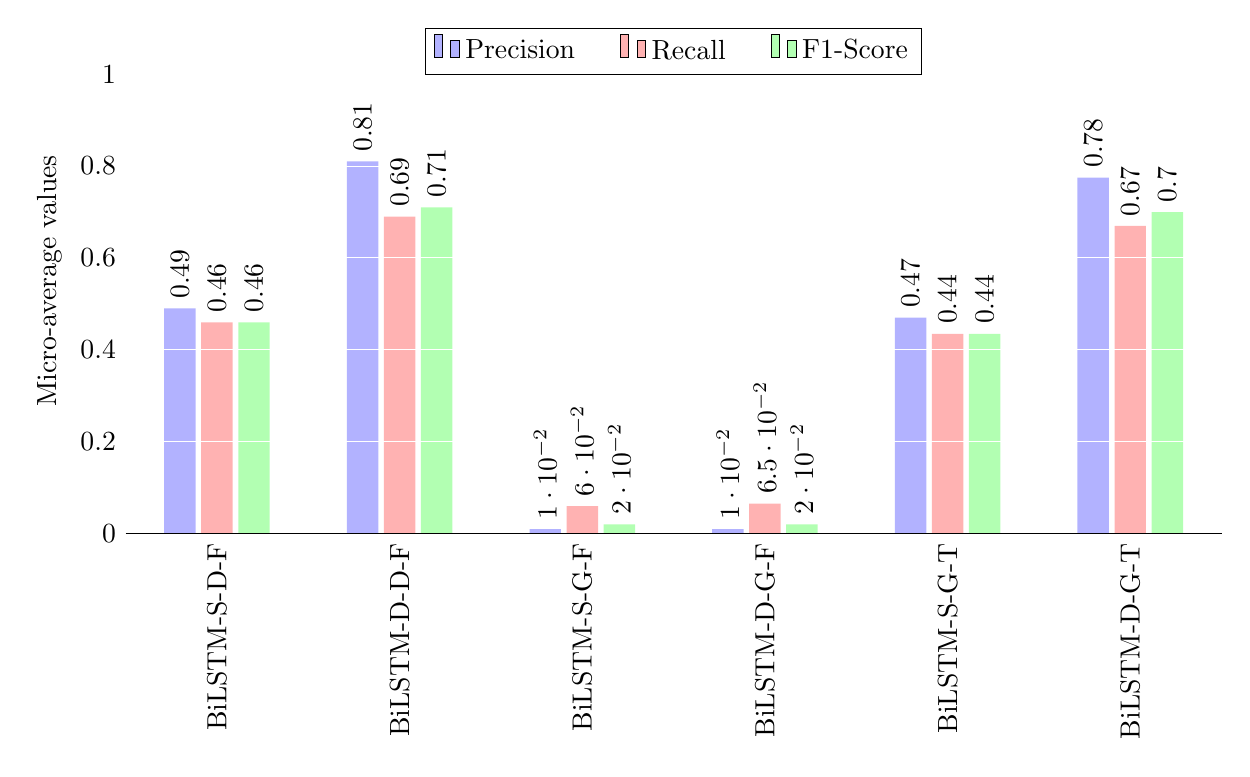
\begin{tikzpicture}
        \centering
  \begin{axis}[
        ybar, axis on top,
        height=8cm, width=15.5cm,
        bar width=0.4cm,
        ymajorgrids, tick align=inside,
        major grid style={draw=white},
        x tick label style={rotate=90,anchor=east},
        enlarge y limits={value=.1,upper},
        ymin=0, ymax=1,
        axis x line*=bottom,
        axis y line*=left,
        y axis line style={opacity=0},
        tickwidth=0pt,
        enlarge x limits=true,
        legend style={
            at={(0.5,1)},
            anchor=north,
            legend columns=-1,
            /tikz/every even column/.append style={column sep=0.5cm}
        },
        ylabel={Micro-average values},
        symbolic x coords=
        {
            BiLSTM-S-D-F,
            BiLSTM-D-D-F,
            BiLSTM-S-G-F,
            BiLSTM-D-G-F,
            BiLSTM-S-G-T,
            BiLSTM-D-G-T
        },
       xtick=data,
       nodes near coords,        
       every node near coord/.append style={color=black,rotate=90, anchor=west }
       %nodes near coords={
       %\pgfmathprintnumber[precision=1]{\pgfplotspointmeta}
       %}
    ]
    \addplot [draw=none, fill=blue!30] coordinates 
    {
        (BiLSTM-S-D-F,0.49)
        (BiLSTM-D-D-F,0.81)
        (BiLSTM-S-G-F,0.01)
        (BiLSTM-D-G-F,0.01)
        (BiLSTM-S-G-T,0.47)
        (BiLSTM-D-G-T,0.775)
    };
   \addplot [draw=none,fill=red!30] coordinates 
   {
        (BiLSTM-S-D-F,0.46)
        (BiLSTM-D-D-F,0.69)
        (BiLSTM-S-G-F,0.06)
        (BiLSTM-D-G-F,0.065)
        (BiLSTM-S-G-T,0.435)
        (BiLSTM-D-G-T,0.67)
   };
   \addplot [draw=none, fill=green!30] coordinates 
   {
        (BiLSTM-S-D-F,0.46)
        (BiLSTM-D-D-F,0.71)
        (BiLSTM-S-G-F,0.02)
        (BiLSTM-D-G-F,0.02)
        (BiLSTM-S-G-T,0.435)
        (BiLSTM-D-G-T,0.7)
    };

    \legend{Precision, Recall, F1-Score}
  \end{axis}
  \end{tikzpicture} 
  \captionsetup{justification=justified,margin=1cm}
    \caption{Macro-average \textit{Precision}, \textit{Recall} and \textit{F1-Score} of \gls{BiLSTM} trained with general-purpose embeddings and domain-specific embeddings. The first suffix S or D indicates the evaluation on sentence or document level, the second suffix D or G represents the domain-specific or general-purpose word embeddings used in the models. The third suffix F or T indicates the status of embedding training, F represents Frozen and T stands for Trainable.}
    \label{fig:SecondEvalQuestionMacro}
\end{figure}



%%%%%%%%%%%%%%%%%%%%%%%%%%%%%%%%%%%%%%%%%%%%%%%%%%%%%%%%%%%%%%%%%%%%%%%%%%%%%%%%%%%%%

%%%%%%%%%%%%%%%%%%%%%%%%%% MACRO AVERAGE Q2%%%%%%%%%%%%%%%%%%%%%%%%%%%%%%%%%%%%%%%%%
\begin{figure}[!ht]

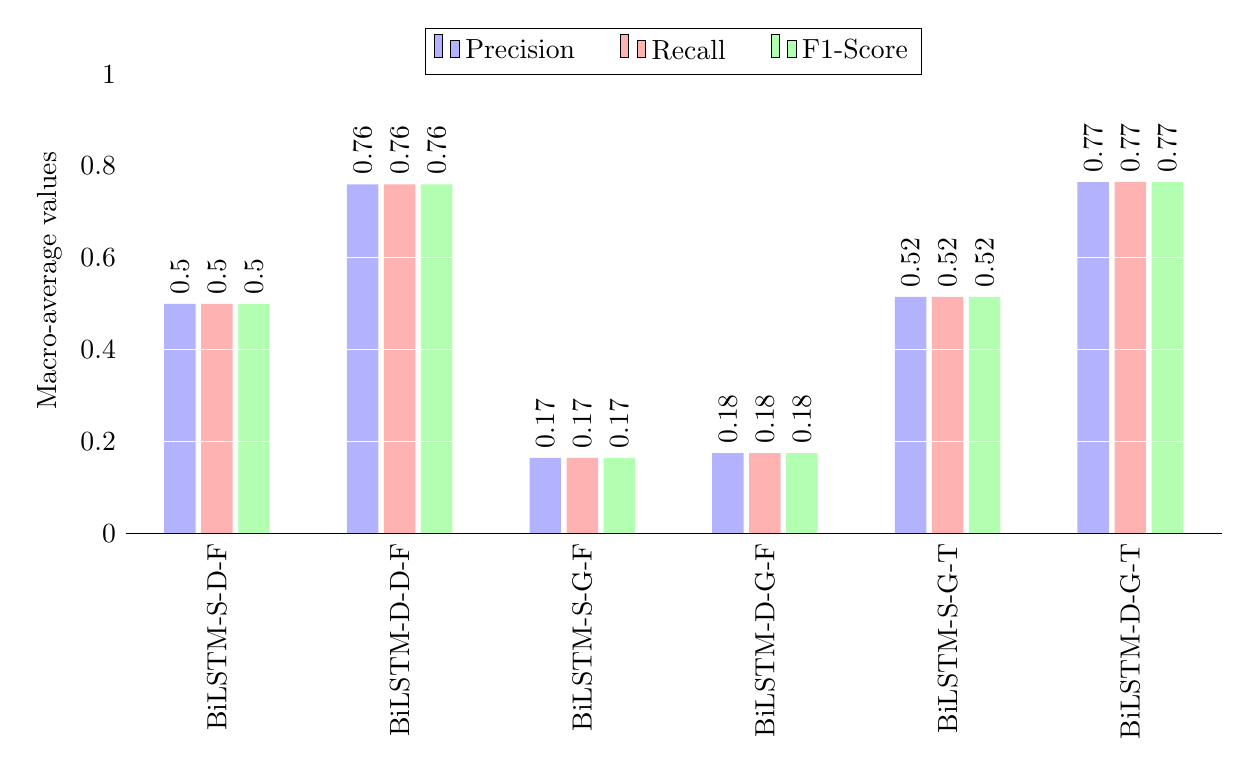
\begin{tikzpicture}
  \centering
  \begin{axis}[
        ybar, axis on top,
        height=8cm, width=15.5cm,
        bar width=0.4cm,
        ymajorgrids, tick align=inside,
        major grid style={draw=white},
        x tick label style={rotate=90,anchor=east},
        enlarge y limits={value=.1,upper},
        ymin=0, ymax=1,
        axis x line*=bottom,
        axis y line*=left,
        y axis line style={opacity=0},
        tickwidth=0pt,
        enlarge x limits=true,
        legend style={
            at={(0.5,1)},
            anchor=north,
            legend columns=-1,
            /tikz/every even column/.append style={column sep=0.5cm}
        },
        ylabel={Macro-average values},
        symbolic x coords=
        {
            BiLSTM-S-D-F,
            BiLSTM-D-D-F,
            BiLSTM-S-G-F,
            BiLSTM-D-G-F,
            BiLSTM-S-G-T,
            BiLSTM-D-G-T
        },
       xtick=data,
       nodes near coords,        
       every node near coord/.append style={color=black,rotate=90, anchor=west }
       %nodes near coords={
       %\pgfmathprintnumber[precision=1]{\pgfplotspointmeta}
      % }
    ]
    \addplot [draw=none, fill=blue!30] coordinates   %Precision
    {
        (BiLSTM-S-D-F,0.5)
        (BiLSTM-D-D-F,0.76)
        (BiLSTM-S-G-F,0.165)
        (BiLSTM-D-G-F,0.175)
        (BiLSTM-S-G-T,0.515)
        (BiLSTM-D-G-T,0.765)
    };
   \addplot [draw=none,fill=red!30] coordinates     % Recall 
   {
        (BiLSTM-S-D-F,0.5)
        (BiLSTM-D-D-F,0.76)
        (BiLSTM-S-G-F,0.165)
        (BiLSTM-D-G-F,0.175)
        (BiLSTM-S-G-T,0.515)
        (BiLSTM-D-G-T,0.765)
   };
   \addplot [draw=none, fill=green!30] coordinates  % F1-Score
   {
        (BiLSTM-S-D-F,0.5)
        (BiLSTM-D-D-F,0.76)
        (BiLSTM-S-G-F,0.165)
        (BiLSTM-D-G-F,0.175)
        (BiLSTM-S-G-T,0.515)
        (BiLSTM-D-G-T,0.765)
    };

    \legend{Precision, Recall, F1-Score}
  \end{axis}
  \end{tikzpicture}
  \captionsetup{justification=justified,margin=1cm}
  \caption{Micro-average \textit{Precision}, \textit{Recall} and \textit{F1-Score} of \gls{BiLSTM} trained with general-purpose embeddings and domain-specific embeddings. The first suffix S or D indicates the evaluation on sentence or document level, the second suffix D or G represents the domain-specific or general-purpose word embeddings used in the models. The third suffix F or T indicates the status of embedding training, F represents Frozen and T stands for Trainable.}
    \label{fig:SecondEvalQuestionMicro}
\end{figure}
%%%%%%%%%%%%%%%%%%%%%%%%%%%%%%%%%%%%%%%%%%%%%%%%%%%%%%%%%%%%%%%%%%%%%%%%%%%%%%%%%%%%%%%%%%%%%%%%%%%%%%%%




%\begin{figure}[!ht]
    %\centering
   % 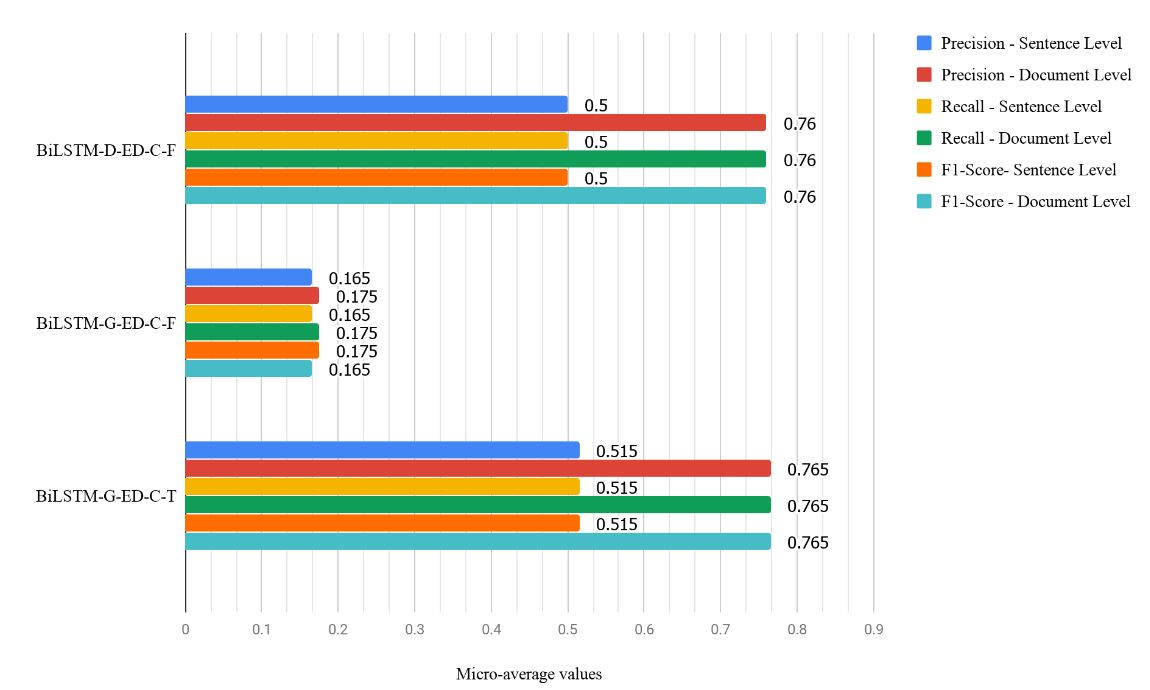
\includegraphics[width=15cm, keepaspectratio]{pics/micro2.jpg}
    %\caption{Micro-average \textit{Precision}, \textit{Recall} and \textit{F1-Score} of \gls{BiLSTM} trained with general-purpose embeddings and domain-specific embeddings. The first suffix D or G represents the domain-specific and general-purpose word embeddings used in the models. The second suffix ED represents the corpus languages English and German, the third suffix C represents that trained is done on clustered data. The fourth suffix F or T indicates the status of embedding training, F represents Frozen and T stands for Trainable. All the models are evaluated on document level and on sentence level}
    %\label{fig:SecondEvalQuestionMicro}
%\end{figure}


%\begin{figure}[!ht]
    %\centering
    %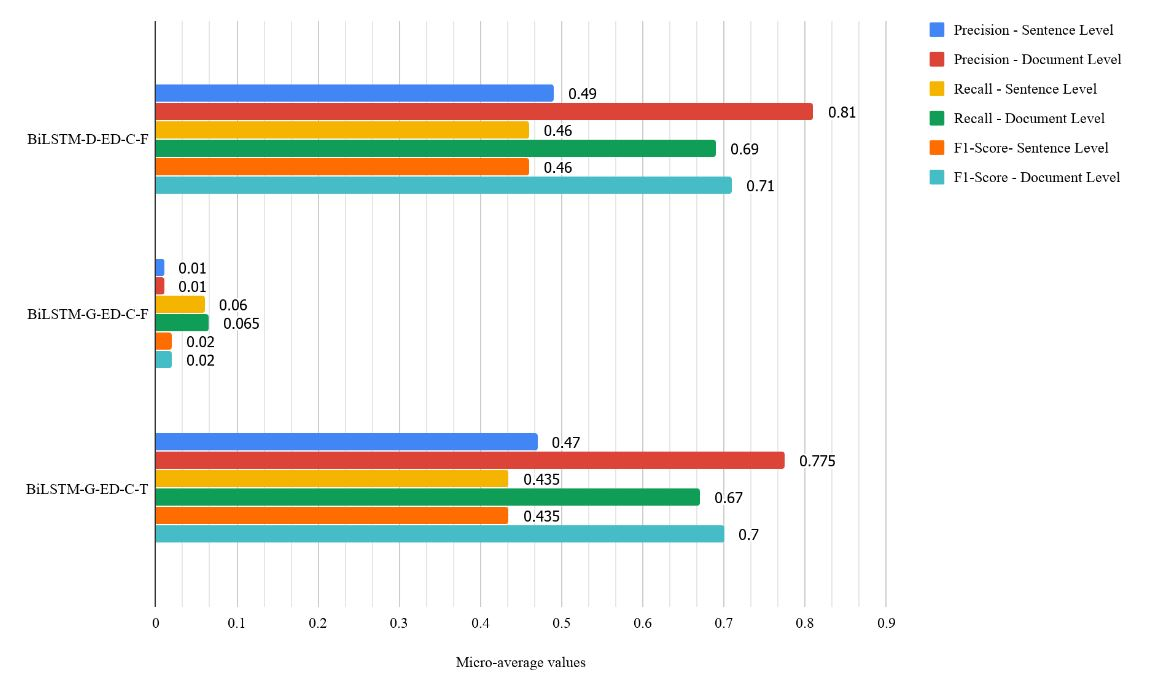
\includegraphics[width=15cm, keepaspectratio]{pics/2.jpg}
    %\caption{Macro-average \textit{Precision}, \textit{Recall} and \textit{F1-Score} of \gls{BiLSTM} trained with general-purpose embeddings and domain-specific embeddings. The first suffix D or G represents the domain-specific and general-purpose word embeddings used in the models. The second suffix ED represents the corpus languages English and German; the third suffix C represents that trained is done on clustered data. The fourth suffix F or T indicates the status of embedding training, F represents Frozen, and T stands for Trainable. All the models are evaluated on the document level and sentence level}
    %\label{fig:SecondEvalQuestionMacro}
%\end{figure}

From \ref{fig:SecondEvalQuestionMicro} and \ref{fig:SecondEvalQuestionMacro} it is quite evident that domain specific word embeddings perform notably better than the general-purpose word embeddings. BiLSTM-D-ED-C-F is the model with domain-specific embedding and has the embedding layer frozen, which means that the embedding layer's weights will not be updated during the training of the network. BiLSTM-G-ED-C-F is the model with frozen general-purpose word embeddings, similar to the previous model; the weights of this model will not be updated. BiLSTM-G-ED-C-T is the model with trainable general-purpose word embeddings, unlike the previous two models, in this model we allow the model to update the weights of the embeddings. This was necessary to evaluate as the general-purpose embeddings are trained on text from sources like Wikipedia or news article, which are not as complex in style and structure compared to legal text. This is the reason as to why it outperformed the model whose embedding weights were frozen. 

The classification models BiLSTM-S-G-F and BiLSTM-D-G-F shown in \ref{fig:SecondEvalQuestionMicro} and \ref{fig:SecondEvalQuestionMacro} performed worst. It overfitted on the data and did predict everything to a single class. One of the reasons for this performance could be that the embedding matrix was never updated. As mentioned above that the general-purpose word embeddings use free text corpus such as Wikipedia and News articles, which contains information about multiple domains. Hence, when these embeddings were trained on Wikipedia and the News article corpus, the semantics captured is different from the one that is specifically trained on the legal corpus. One example of this can be seen in Image Recognition task when applying transfer learning; it is advisable that the dataset for prediction or classification task being performed should be similar to the ones we are doing transfer learning from \cite{iglovikov2018ternausnet}.

Another reason is that general-purpose word embeddings do not contain specialized words that are used in the legal domain. The EUR-lex summaries of English and German corpus for cluster 1 data contains 43339 words and when the embedding matrix is created only 20310 words were found in the general-purpose embedding. That is only half of the words. So training the general-purpose embeddings is necessary to get better performance which can be seen from the \ref{fig:SecondEvalQuestionMacro}.

The visualization randomly selected 10 words of general-purpose embeddings before training (which is the visualization of frozen word embedding) and after training (which is a visualization of trained word embedding) is in \ref{visualEmb}. 

The results are comparable. The \ref{table:Evaal2} shows in detail the class-wise precision, recall, and f1-score of \gls{BiLSTM} trained on English and German corpus with the general-purpose word embeddings and on the domain-specific word embeddings.

% Please add the following required packages to your document preamble:
% \usepackage[normalem]{ulem}
% \useunder{\uline}{\ul}{}
\begin{table}[!ht]
\begin{tabular}{>{\raggedright\arraybackslash}m{5.8cm}>{\centering\arraybackslash}m{1cm}>{\centering\arraybackslash}m{1cm}>{\centering\arraybackslash}m{1cm}>{\centering\arraybackslash}m{1.1cm}>{\centering\arraybackslash}m{1.1cm}>{\centering\arraybackslash}m{1.1cm}}
\hline
Category & P$_\text{\tiny{LSTM-D}}$ &  R$_\text{\tiny{LSTM-D}}$ & F$_\text{\tiny{LSTM-D}}$ & P$_\text{\tiny{LSTM-G}}$ & R$_\text{\tiny{LSTM-G}}$ & F$_\text{\tiny{LSTM-C}}$ \\ \hline
Agriculture & \hlc[precision]{ 0.90} & \hlc[recall]{0.86} & \hlc[fscore]{0.88} & 0.82 & 0.80 & 0.81 \\
Audiovisual and Media & \hlc[precision]{ 1.00} & \hlc[recall]{0.10} & \hlc[fscore]{0.18} & 0.00 & 0.00 & 0.00 \\
Budget & \hlc[precision]{ 0.78} & \hlc[recall]{0.70} & \hlc[fscore]{0.74} & 0.67 & 0.20 & 0.31 \\
Competition & \hlc[precision]{ 0.96} & 0.83 & \hlc[fscore]{0.89} & 0.89 & 0.83 & 0.86 \\
Consumers & 0.59 & \hlc[recall]{0.65} & 0.62 & \hlc[precision]{ 0.65} & 0.65 & \hlc[fscore]{0.65} \\
Culture & 0.93 & \hlc[recall]{1.00} & \hlc[fscore]{0.97} & \hlc[precision]{ 1.00} & 0.50 & 0.67 \\
Customs & 0.64 & \hlc[recall]{0.70} & 0.67 & \hlc[precision]{ 0.94} & 0.53 & \hlc[fscore]{0.68} \\
Development & 0.64 & \hlc[recall]{0.83} & 0.72 & \hlc[precision]{ 0.64} & 0.81 & 0.72 \\
Economic and Monetary Affairs & \hlc[precision]{ 0.95} & 0.87 & 0.91 & 0.90 & \hlc[recall]{0.95} & \hlc[fscore]{0.93} \\
Education Training Youth & 0.86 & 0.94 & 0.90 & \hlc[precision]{ 0.91} & 0.94 & \hlc[fscore]{0.92} \\
Employment and Social Policy & 0.71 & \hlc[recall]{0.88} & \hlc[fscore]{0.79} & 0.71 & 0.86 & 0.78 \\
Energy & 0.97 & 0.64 & 0.77 & \hlc[precision]{ 0.98} & \hlc[recall]{0.71} & \hlc[fscore]{0.82} \\
Enlargement & \hlc[precision]{ 0.76} & 0.59 & \hlc[fscore]{0.67} & 0.65 & \hlc[recall]{0.62} & 0.63 \\
Enterprise & \hlc[precision]{ 0.65} & \hlc[recall]{0.42} & \hlc[fscore]{0.51} & 0.64 & 0.35 & 0.45 \\
Environment & 0.70 & 0.84 & 0.76 & \hlc[precision]{ 0.80} & \hlc[recall]{0.89} & \hlc[fscore]{0.84} \\
External Relations & \hlc[precision]{ 0.92} & 0.55 & \hlc[fscore]{0.69} & 0.68 & \hlc[recall]{0.59} & 0.63 \\
External Trade & 0.61 & \hlc[recall]{0.71} & \hlc[fscore]{0.66} & \hlc[precision]{ 0.72} & 0.46 & 0.57 \\
Fight Against Fraud & 0.53 & \hlc[recall]{0.50} & \hlc[fscore]{0.52} & \hlc[precision]{ 0.83} & 0.31 & 0.45 \\
Food Safety & \hlc[precision]{ 0.93} & 0.82 & \hlc[fscore]{0.87} & 0.84 & \hlc[recall]{0.87} & 0.85 \\
Foreign and Security Policy & 0.62 & \hlc[recall]{0.83} & \hlc[fscore]{0.71} & \hlc[precision]{ 0.79} & 0.62 & 0.70 \\
Human Rights & 0.59 & \hlc[recall]{0.71} & \hlc[fscore]{0.64} & \hlc[precision]{ 0.89} & 0.33 & 0.48 \\
Humanitarian Aid & 0.67 & 0.57 & 0.62 & \hlc[precision]{ 1.00} & 0.57 & \hlc[fscore]{0.73} \\
Information Society & 0.71 & 0.84 & 0.77 & \hlc[precision]{ 0.76} & \hlc[recall]{0.90} & \hlc[fscore]{0.82} \\
Institutional Affairs & \hlc[precision]{ 0.67} & 0.65 & \hlc[fscore]{0.66} & 0.55 & \hlc[recall]{0.80} & 0.65 \\
Internal Market & 0.72 & 0.75 & 0.74 & \hlc[precision]{ 0.74} & \hlc[recall]{0.80} & \hlc[fscore]{0.77} \\
Justice Freedom Security & \hlc[precision]{ 0.81} & 0.67 & 0.74 & 0.69 & \hlc[recall]{0.89} & \hlc[fscore]{0.78} \\
Maritime Affairs and Fisheries & \hlc[precision]{ 0.94} & \hlc[recall]{0.91} & \hlc[fscore]{0.92} & 0.87 & 0.89 & 0.88 \\
Public Health & 0.86 & 0.43 & 0.58 & \hlc[precision]{ 0.92} & \hlc[recall]{0.52} & \hlc[fscore]{0.67} \\
Regional Policy & 0.72 & 0.86 & 0.78 & \hlc[precision]{ 0.81} & \hlc[recall]{0.90} & \hlc[fscore]{0.85} \\
Research Innovation & 0.60 & \hlc[recall]{0.96} & 0.74 & \hlc[precision]{ 0.79} & 0.79 & \hlc[fscore]{0.79} \\
Taxation & 0.95 & \hlc[recall]{0.71} & \hlc[fscore]{0.82} & 0.95 & 0.64 & 0.77 \\
Transport & 0.76 & 0.86 & 0.81 & \hlc[precision]{ 0.82} & \hlc[recall]{0.89} & \hlc[fscore]{0.85} \\ \hline
\end{tabular}
\captionsetup{justification=justified,margin=1cm}
\caption{Class-wise precision (P) and recall (R) and F1-Score (F) for BiLSTM-D-ED-C-T (represented with suffix LSTM-D) and BiLSTM-D-ED-C-T (represented with suffix LSTM-G) on evaluated on document level. The best \textit{precision}, \textit{recall} and \textit{f1-scores} among both the classifiers is highlighted in \hlc[precision]{blue}, \hlc[recall]{red} and \hlc[fscore]{green} respectively. If the values across both the classifiers are same it not highlighted.}

\label{table:Evaal2}
\end{table}

As we can see from the \ref{table:Evaal2} the performance of domain-specific word embeddings is better in general compared to the general-purpose embeddings. For the class \textit{Audiovisual and Media}, general-purpose embeddings did not classify a single document. 
\clearpage

\subsection{Evaluation for third research question}

The third research question investigates the effect of having a multilingual parallel corpus on the classification task. A multilingual parallel corpus here means having different language documents for a predefined category. 

As described in \ref{fig:FlowResearchQuestion2} two \glspl{BiLSTM} classification models, one trained with English corpus and other trained with German corpus are compared with a single \gls{BiLSTM} classification model trained on English and German corpus.

\begin{figure}[!ht]
    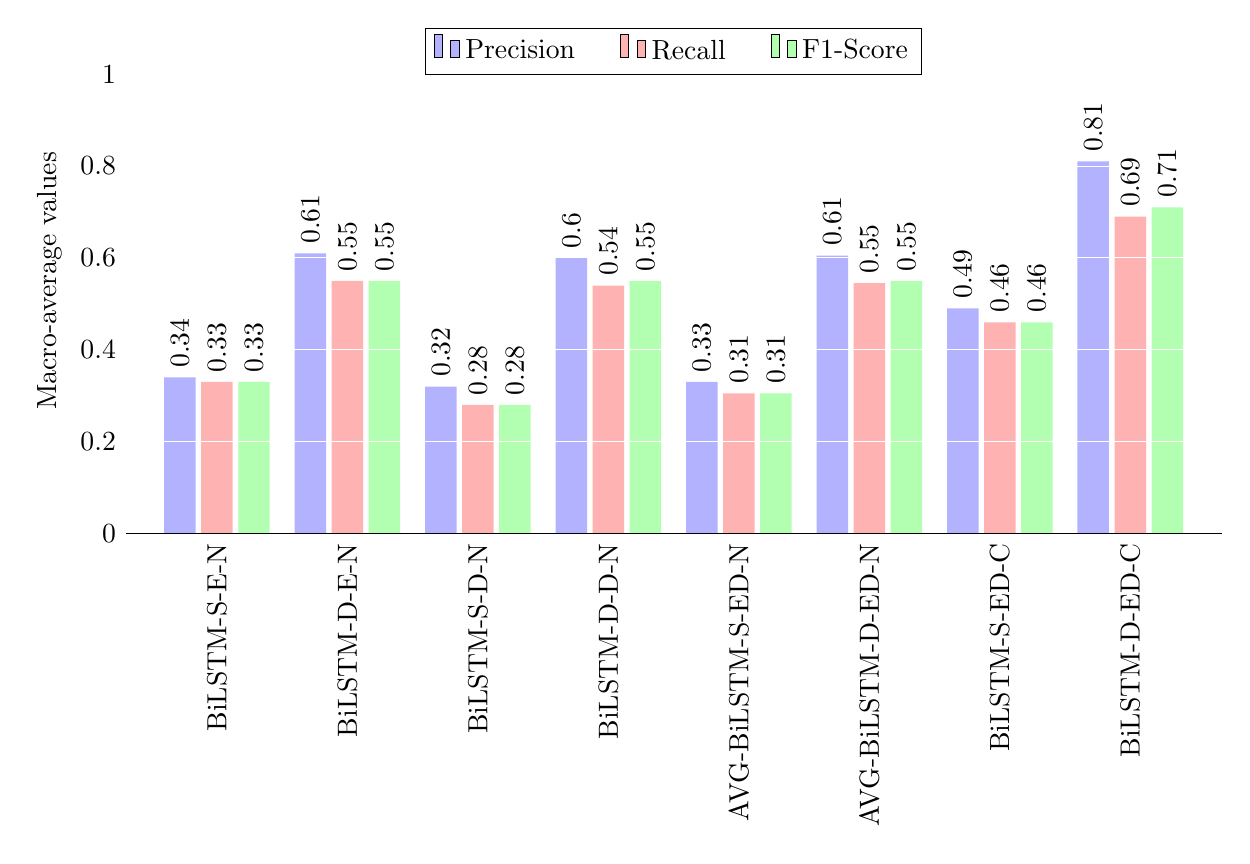
\begin{tikzpicture}
  \centering
  \begin{axis}[
        ybar, axis on top,
        height=8cm, width=15.5cm,
        bar width=0.4cm,
        ymajorgrids, tick align=inside,
        major grid style={draw=white},
        x tick label style={rotate=90,anchor=east},
        enlarge y limits={value=.1,upper},
        ymin=0, ymax=1,
        axis x line*=bottom,
        axis y line*=left,
        y axis line style={opacity=0},
        tickwidth=0pt,
        enlarge x limits=true,
        legend style={
            at={(0.5,1)},
            anchor=north,
            legend columns=-1,
            /tikz/every even column/.append style={column sep=0.5cm}
        },
        ylabel={Macro-average values},
        symbolic x coords=
        {
            BiLSTM-S-E-N,
            BiLSTM-D-E-N,
            BiLSTM-S-D-N,
            BiLSTM-D-D-N,
            AVG-BiLSTM-S-ED-N,
            AVG-BiLSTM-D-ED-N,
            BiLSTM-S-ED-C,
            BiLSTM-D-ED-C
        },
       xtick=data,
       nodes near coords,        
       every node near coord/.append style={color=black,rotate=90, anchor=west }
       %nodes near coords={
       %\pgfmathprintnumber[precision=1]{\pgfplotspointmeta}
       %}
    ]
    \addplot [draw=none, fill=blue!30] coordinates   %Precision
    {
        (BiLSTM-S-E-N,0.34)
        (BiLSTM-D-E-N,0.61)
        (BiLSTM-S-D-N,0.32)
        (BiLSTM-D-D-N,0.6)
        (AVG-BiLSTM-S-ED-N,0.33)
        (AVG-BiLSTM-D-ED-N,0.605)
        (BiLSTM-S-ED-C,0.49)
        (BiLSTM-D-ED-C,0.81)
    };
   \addplot [draw=none,fill=red!30] coordinates     % Recall 
   {
       (BiLSTM-S-E-N,0.33)
       (BiLSTM-D-E-N,0.55)
       (BiLSTM-S-D-N,0.28)
       (BiLSTM-D-D-N,0.54)
       (AVG-BiLSTM-S-ED-N,0.305)
       (AVG-BiLSTM-D-ED-N,0.545)
       (BiLSTM-S-ED-C,0.46)
       (BiLSTM-D-ED-C,0.69)
   };
   \addplot [draw=none, fill=green!30] coordinates  % F1-Score
   {        
        (BiLSTM-S-E-N,0.33)
        (BiLSTM-D-E-N,0.55)
        (BiLSTM-S-D-N,0.28)
        (BiLSTM-D-D-N,0.55)
        (AVG-BiLSTM-S-ED-N,0.305)
        (AVG-BiLSTM-D-ED-N,0.55)
        (BiLSTM-S-ED-C,0.46)
        (BiLSTM-D-ED-C,0.71)
    };

    \legend{Precision, Recall, F1-Score}
  \end{axis}
  \end{tikzpicture}  
  \captionsetup{justification=justified,margin=1cm}
    \caption{Macro-average \textit{Precision}, \textit{Recall} and \textit{F1-Score} for \gls{BiLSTM}. The first suffix specifies the method of evaluation (S = Sentence and D = Document), the suffix second E, D or ED specifies the language of the corpus, English, German or both English and German respectively. The second suffix N or C represents that model is trained on non clustered or clustered data respectively. AVG-BiLSTM-ED-N represents the average score from BiLSTM-E-N and BiLSTM-D-N}
    \label{fig:EvaluationQuestion3Macro}
\end{figure}

%%%%%%%%%%%%%%%%%%%%%%%%%%%%%%%%%%%%%%%%%%%%%%%%%%%%%%%%%%%%%%%%%%%%%%%%%%%%%%%%%%%%%%%%%%%%%

%%%%%%%%%%%%%%%%%%%%%%%%%%%% MACRO Q3%%%%%%%%%%%%%%%%%%%%%%%%%%%%%%%%%%%%%%%%%%%%%%%%%%%%%%%%%

\begin{figure}[!ht]
    \centering
    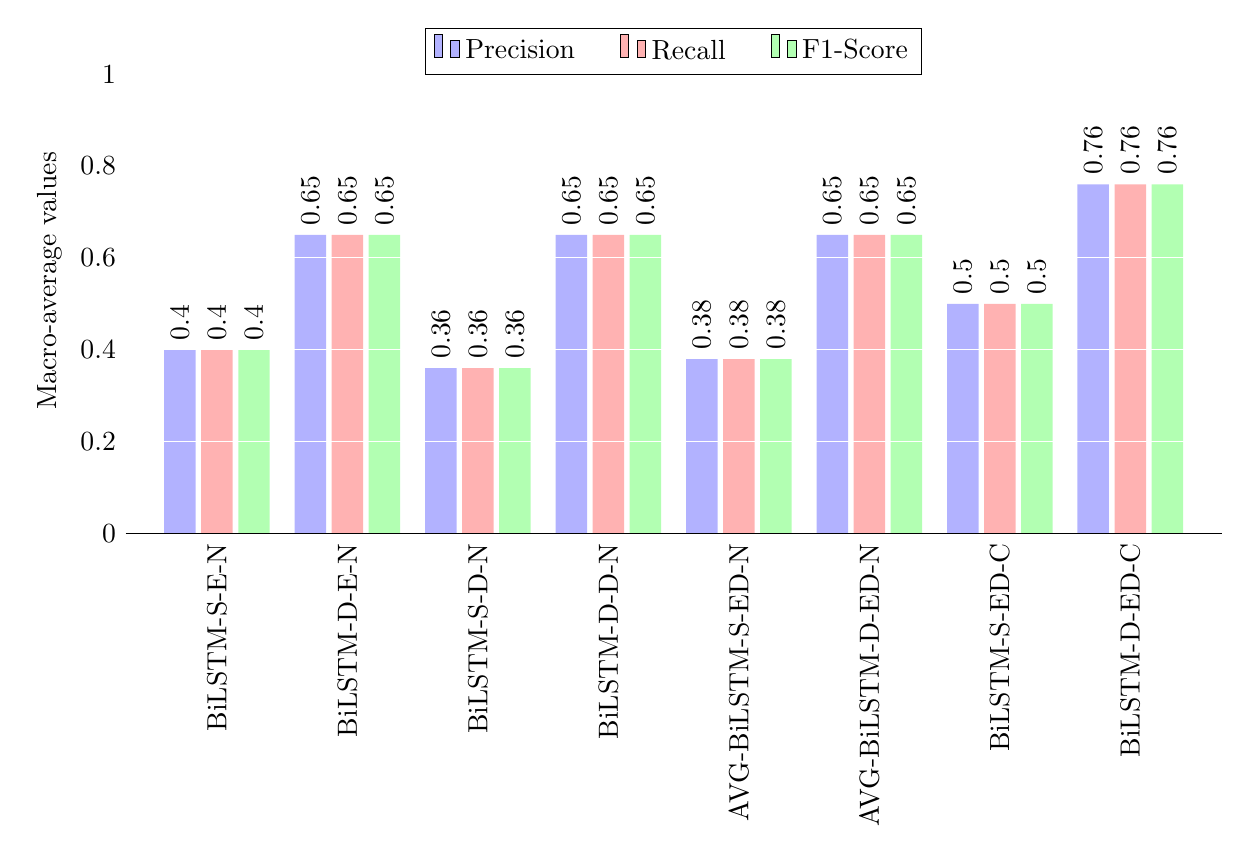
\begin{tikzpicture}
  \centering
  \begin{axis}[
        ybar, axis on top,
        height=8cm, width=15.5cm,
        bar width=0.4cm,
        ymajorgrids, tick align=inside,
        major grid style={draw=white},
        x tick label style={rotate=90,anchor=east},
        enlarge y limits={value=.1,upper},
        ymin=0, ymax=1,
        axis x line*=bottom,
        axis y line*=left,
        y axis line style={opacity=0},
        tickwidth=0pt,
        enlarge x limits=true,
        legend style={
            at={(0.5,1)},
            anchor=north,
            legend columns=-1,
            /tikz/every even column/.append style={column sep=0.5cm}
        },
        ylabel={Macro-average values},
        symbolic x coords=
        {
            BiLSTM-S-E-N,
            BiLSTM-D-E-N,
            BiLSTM-S-D-N,
            BiLSTM-D-D-N,
            AVG-BiLSTM-S-ED-N,
            AVG-BiLSTM-D-ED-N,
            BiLSTM-S-ED-C,
            BiLSTM-D-ED-C
        },
       xtick=data,
       nodes near coords,        
       every node near coord/.append style={color=black,rotate=90, anchor=west }
       %nodes near coords={
       %\pgfmathprintnumber[precision=1]{\pgfplotspointmeta}
       %}
    ]
    \addplot [draw=none, fill=blue!30] coordinates 
    {
            (BiLSTM-S-E-N,0.4)
            (BiLSTM-D-E-N,0.65)
            (BiLSTM-S-D-N,0.36)
            (BiLSTM-D-D-N,0.65)
            (AVG-BiLSTM-S-ED-N,0.38)
            (AVG-BiLSTM-D-ED-N,0.65)
            (BiLSTM-S-ED-C,0.5)
            (BiLSTM-D-ED-C,0.76)
    };
   \addplot [draw=none,fill=red!30] coordinates 
   {
            (BiLSTM-S-E-N,0.4)
            (BiLSTM-D-E-N,0.65)
            (BiLSTM-S-D-N,0.36)
            (BiLSTM-D-D-N,0.65)
            (AVG-BiLSTM-S-ED-N,0.38)
            (AVG-BiLSTM-D-ED-N,0.65)
            (BiLSTM-S-ED-C,0.5)
            (BiLSTM-D-ED-C,0.76)
   };
   \addplot [draw=none, fill=green!30] coordinates 
   {
            (BiLSTM-S-E-N,0.4)
            (BiLSTM-D-E-N,0.65)
            (BiLSTM-S-D-N,0.36)
            (BiLSTM-D-D-N,0.65)
            (AVG-BiLSTM-S-ED-N,0.38)
            (AVG-BiLSTM-D-ED-N,0.65)
            (BiLSTM-S-ED-C,0.5)
            (BiLSTM-D-ED-C, 0.76)
    };

    \legend{Precision, Recall, F1-Score}
  \end{axis}
  \end{tikzpicture} 
  \captionsetup{justification=justified,margin=1cm}
    \caption{Micro-average \textit{Precision}, \textit{Recall} and \textit{F1-Score} for \gls{BiLSTM}. The first suffix specifies the method of evaluation (S = Sentence and D = Document), the suffix second E, D or ED specifies the language of the corpus, English, German or both English and German respectively. The second suffix N or C represents that model is trained on non clustered or clustered data respectively. AVG-BiLSTM-ED-N represents the average score from BiLSTM-E-N and BiLSTM-D-N}
    \label{fig:EvaluationQuestion3Micro}
\end{figure}

%%%%%%%%%%%%%%%%%%%%%%%%%%%%%%%%%%%%%%%%%%%%%%%%%%%%%%%%%%%%%%%%%%%%%%%%%%%%%%%%%%%%%%%%%%%%%
%\begin{figure}[!ht]
    %\centering
    %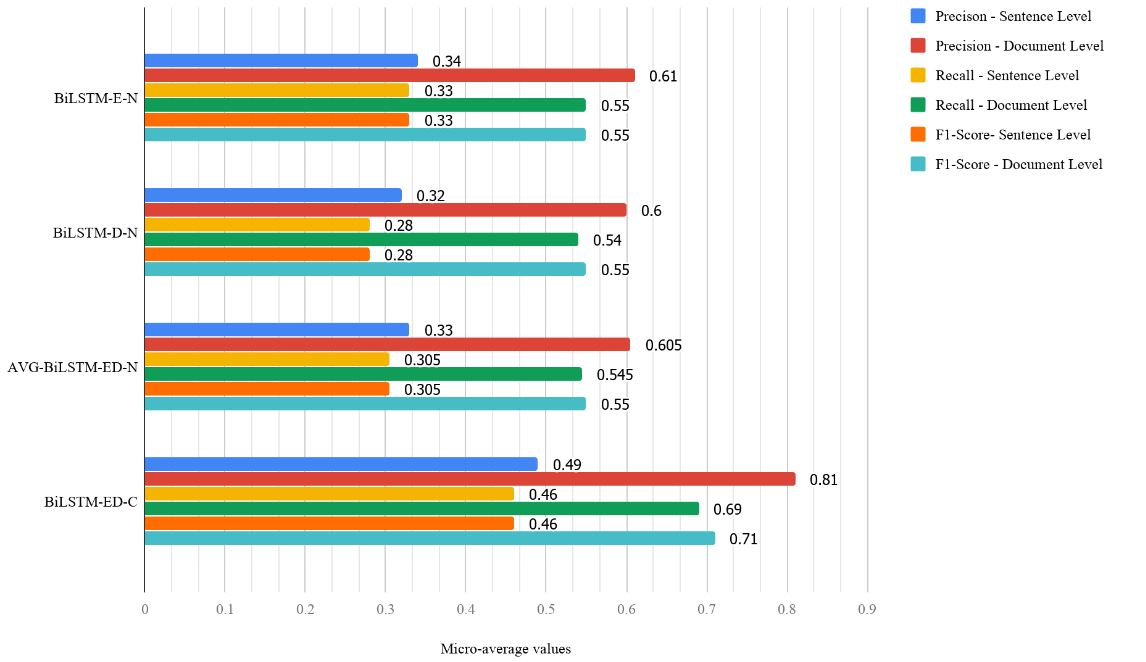
\includegraphics[width=15cm, keepaspectratio]{pics/3.jpg}
    %\caption{Macro-average \textit{Precision}, \textit{Recall} and \textit{F1-Score} for \gls{BiLSTM} trained on English corpus and German corpus separately and together. The suffix first E, D or ED specifies the language of the corpus, English, German or both English and German respectively. The second suffix N or C represents that model is trained on non clustered or clustered data respectively. AVG-BiLSTM-ED-N represents the average score from BiLSTM-E-N and BiLSTM-D-N}
    %\label{fig:EvaluationQuestion3}
%\end{figure}

\ref{fig:EvaluationQuestion3Macro} shows the macro-average precision, recall, and f1-scores indicate that employing a single classifier for the bilingual corpus is considerably better than two different classifiers for two different languages. \ref{fig:EvaluationQuestion3Macro} also confirms the above mentioned statement.
One explanation for the better performance of the bilingual classifier is that it has more example to learn from than the previous case. C.-P. Wei et al. showed that polylingual data could be used to increase the performance of a classifier \cite{Wei:2014:EPD:2566999.2567111}. Also, the clustering of the data would have helped as compared to unclustered data as shown in \ref{tabel:LSTMCluster&NonClustered} and  \ref{fig:question1EvalMicro}. 


The class-wise precision, recall, and f1-scores of classifiers AVG-BiLSTM-ED-N and BiLSTM-ED-C is show in \ref{tabel:Eval3}

% Please add the following required packages to your document preamble:
% \usepackage[normalem]{ulem}
% \useunder{\uline}{\ul}{}
\begin{table}[!ht]
\centering
\begin{tabular}{>{\raggedright\arraybackslash}m{5.8cm}>{\centering\arraybackslash}m{1cm}>{\centering\arraybackslash}m{1cm}>{\centering\arraybackslash}m{1cm}>{\centering\arraybackslash}m{1.1cm}>{\centering\arraybackslash}m{1.1cm}>{\centering\arraybackslash}m{1.1cm}}
\hline
Category & P$_\text{\tiny{LSTM-A}}$ &  R$_\text{\tiny{LSTM-A}}$ & F$_\text{\tiny{LSTM-A}}$ & P$_\text{\tiny{LSTM-B}}$ & R$_\text{\tiny{LSTM-B}}$ & F$_\text{\tiny{LSTM-B}}$ \\ \hline
Agriculture & 0.65 & 0.82 & 0.72 & \hlc[precision]{ 0.90} & \hlc[recall]{0.86} & \hlc[fscore]{0.88} \\
Audiovisual and Media & 0.00 & 0.00 & 0.00 & \hlc[precision]{ 1.00} & \hlc[recall]{0.10} & \hlc[fscore]{0.18} \\
Budget & 0.00 & 0.00 & 0.00 & \hlc[precision]{ 0.78} & \hlc[recall]{0.70} & \hlc[fscore]{0.74} \\
Competition & 0.50 & 0.16 & 0.25 & \hlc[precision]{ 0.96} & \hlc[recall]{0.83} & \hlc[fscore]{0.89} \\
Consumers & 0.57 & 0.62 & 0.60 & \hlc[precision]{ 0.59} & \hlc[recall]{0.65} & \hlc[fscore]{0.62} \\
Culture & 0.61 & 0.57 & 0.53 & \hlc[precision]{ 0.93} & \hlc[recall]{1.00} & \hlc[fscore]{0.97} \\
Customs & 0.68 & 0.05 & 0.58 & \hlc[precision]{ 0.64} & \hlc[recall]{0.70} & \hlc[fscore]{0.67} \\
Development & 0.60 & 0.77 & 0.67 & \hlc[precision]{ 0.64} & \hlc[recall]{0.83} & \hlc[fscore]{0.72} \\
Economic and Monetary Affairs & 0.91 & \hlc[recall]{0.93} & 0.92 & \hlc[precision]{ 0.95} & 0.87 & \hlc[fscore]{0.91} \\
Education Training Youth & 0.77 & 0.88 & 0.82 & \hlc[precision]{ 0.86} & \hlc[recall]{0.94} & \hlc[fscore]{0.90} \\
Employment and Social Policy & 0.62 & 0.78 & 0.69 & \hlc[precision]{ 0.71} & \hlc[recall]{0.88} & \hlc[fscore]{0.79} \\
Energy & 0.76 & 0.61 & 0.67 & \hlc[precision]{ 0.97} & \hlc[recall]{0.64} & \hlc[fscore]{0.77} \\
Enlargement & 0.53 & 0.53 & 0.53 & \hlc[precision]{ 0.76} & \hlc[recall]{0.59} & \hlc[fscore]{0.67} \\
Enterprise & 0.19 & 0.23 & 0.20 & \hlc[precision]{ 0.65} & \hlc[recall]{0.42} & \hlc[fscore]{0.51} \\
Environment & 0.62 & 0.80 & 0.70 & \hlc[precision]{ 0.70} & \hlc[recall]{0.84} & \hlc[fscore]{0.76} \\
External Relations & 0.73 & 0.36 & 0.48 & \hlc[precision]{ 0.92} & \hlc[recall]{0.55} & \hlc[fscore]{0.69} \\
External Trade & 0.47 & 0.64 & 0.53 & \hlc[precision]{ 0.61} & \hlc[recall]{0.71} & \hlc[fscore]{0.66} \\
Fight Against Fraud & 0.40 & 0.25 & 0.31 & \hlc[precision]{ 0.53} & \hlc[recall]{0.50} & \hlc[fscore]{0.52} \\
Food Safety & \hlc[precision]{ 0.95} & 0.75 & 0.85 & 0.93 & \hlc[recall]{0.82} & \hlc[fscore]{0.87} \\
Foreign and Security Policy & 0.57 & 0.50 & 0.53 & \hlc[precision]{ 0.62} & \hlc[recall]{0.83} & \hlc[fscore]{0.71} \\
Human Rights & \hlc[precision]{ 1.00} & 0.25 & 0.39 & 0.59 & \hlc[recall]{0.71} & \hlc[fscore]{0.64} \\
Humanitarian Aid & \hlc[precision]{ 1.00} & 0.36 & 0.52 & 0.67 & \hlc[recall]{0.57} & \hlc[fscore]{0.62} \\
Information Society & 0.62 & 0.68 & 0.65 & \hlc[precision]{ 0.71} & \hlc[recall]{0.84} & \hlc[fscore]{0.77} \\
Institutional Affairs & 0.48 & 0.70 & 0.56 & \hlc[precision]{ 0.67} & \hlc[recall]{0.65} & \hlc[fscore]{0.66} \\
Internal Market & 0.69 & 0.65 & 0.67 & \hlc[precision]{ 0.72} & \hlc[recall]{0.75} & \hlc[fscore]{0.74} \\
Justice Freedom Security & 0.61 & 0.85 & 0.71 & \hlc[precision]{ 0.81} & \hlc[recall]{0.67} & \hlc[fscore]{0.74} \\
Maritime Affairs and Fisheries & 0.84 & 0.81 & 0.82 & \hlc[precision]{ 0.94} & \hlc[recall]{0.91} & \hlc[fscore]{0.92} \\
Public Health & 0.37 & 0.13 & 0.20 & \hlc[precision]{ 0.86} & \hlc[recall]{0.43} & \hlc[fscore]{0.58} \\
Regional Policy & 0.62 & 0.55 & 0.57 & \hlc[precision]{ 0.72} & \hlc[recall]{0.86} & \hlc[fscore]{0.78} \\
Research Innovation & 0.46 & 0.43 & 0.44 & \hlc[precision]{ 0.60} & \hlc[recall]{0.96} & \hlc[fscore]{0.74} \\
Taxation & 0.85 & 0.57 & 0.65 & \hlc[precision]{ 0.95} & \hlc[recall]{0.71} & \hlc[fscore]{0.82} \\
Transport & 0.65 & 0.71 & 0.68 & \hlc[precision]{ 0.76} & \hlc[recall]{0.86} & \hlc[fscore]{0.81} \\ \hline
\end{tabular}
\captionsetup{justification=justified,margin=1cm}
\caption{Class-wise precision (P) and recall (R) and F1-Score (F) for AVG-BiLSTM-ED-N (represented with suffix LSTM-A) and BiLSTM-ED-C (represented with suffix LSTM-B) on evaluated on document level. The best \textit{precision}, \textit{recall} and \textit{f1-scores} among both the classifiers is highlighted in \hlc[precision]{blue}, \hlc[recall]{red} and \hlc[fscore]{green} respectively. If the values across both the classifiers are same it not highlighted.}
\label{tabel:Eval3}
\end{table}

The effects of having multiple languages for training is clear from the \ref{tabel:Eval3}. For classes \textit{Audiovisual and Media} and \textit{Budget} the classifier with a single language in training did not predict a single sample during testing. However, when another language is added to the training data, classification shows signs of improvement. The improvement is significant in case of class \textit{Budget} when for a classifier with a single language the precision, recall and f1-score was 0.00 and for bilingual classifier the precision, recall, and f1-score is 0.78, 0.70 and 0.74 respectively.